A study of the cosmic ray background as a function of the fibre diameter was carried out. Simulations of a single $20~\cm$ length scintillating fibre of $1~\mm$ and $2~\mm$ were compared. The energy deposited in the scintillating fibres by cosmic rays is proportional to the active volume so, the expected cosmic ray signal is larger for $2~\mm$ diameter fibres. The objective of this study is to simulate the background in the tritium energy range. The tritiated water source was replaced by a cosmic ray source generated by the CRY library\footnote{CRY library, Cosmic-Ray Shower library} \cite{CRYwebsite, CRYpaper}, a package implemented in C++. This library generates cosmic-ray showers for different particles (muons, neutrons, protons, electrons, photons and pions). The cosmic source employed is a horizontal square of $1 \times 1~\meter ^2$ located $35~\cm$ over the detector with the typical distribution of cosmic particles at sea level. The distributions of energy deposited in the scintillating fibres for $1~\mm$ and $2~\mm$ diameters by cosmic rays are shown in Figure \ref{fig:DiameterComparison}. As can be seen in the figure, a background about $50\%$ smaller is obtained for $1~\mm$ fibre diameter in the tritium energy range, which implies a smaller detector MDA. %There are other reasons that may favor $2~\mm$ fibres, such as their greater rigidity and better flow of water through them. Thus, a complementary experimental study is needed to assess the most appropriate scintillating fibres diameter.

\begin{figure}[hbtp]
\centering
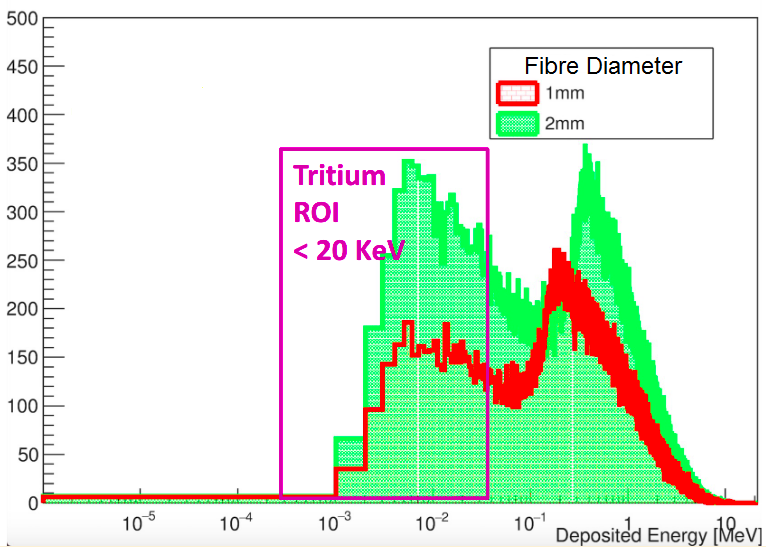
\includegraphics[scale=0.4]{6Simulations/61TRITIUMDesign/614Diameter/ComparisonDiameter.png}
\caption{Comparison of the energy deposition by cosmic rays in scintillating fibres of $1~\mm$ and $2~\mm$ diameter \cite{SimulationPaperCarlos}.\label{fig:DiameterComparison}}
\end{figure}